
\section{Introduction}
\label{sec:introduction}
%%% General intro

\IEEEPARstart{T}{he} constant research and the rapid evolution of machine learning (ML) techniques for sensor data analytics represent a promising landscape for \REVIEW{edge computing and} Internet-of-Things (IoT) endpoint applications. CNN-based models represent the essential building blocks in 2D pattern recognition tasks. Sensor-based applications such as mechanical fault diagnosis\cite{li2019sensor,dong2018rolling}, structural health monitoring (SHM)\cite{nagayama2007structural}, human activity recognition (HAR) \cite{wang2019deep}, hazardous gas detection\cite{kim2017hazardous} have been powered by CNN-based models in industry and academia.

\REVIEW
{
In recent years, there is an increasing demand to introduce on-chip AI-based analytics into the smart city and Industry 4.0 infrastructure \mbox{\cite{lom2016industry}}. The paradigm of edge computing provides new solutions by bringing intelligence closer to the data source. This approach preserves sensitive and private data on devices, and provides low latency, energy efficiency, and scalability compared to cloud services while reducing the network bandwidth \mbox{\cite{chen2019deep}}. Moreover, these solutions are boosted by advances in ML models, processing power, and big data.

CNN-based models, as one of the main types of artificial neural networks (ANNs),
have been successfully used in sensor analytics with automatic feature learning from sensory data \mbox{\cite{ince2016real, janssens2016convolutional, abdeljaber2017real, guo2016hierarchical}}. In this context, CNN models are applied for automatic feature learning, mostly, from 1D time series signals as well as for 2D time-frequency spectrograms. CNN models provide advantages over other methods, such as local dependency and scale invariance. However, these models represent computationally-intensive and power-hungry tasks, particularly, for embedded system architectures.
}

Due to the high computational demands of CNNs, dedicated hardware \REVIEW{architectures are} typically required to accelerate execution \REVIEW{and improve power efficiency}. In terms of computational throughput, graphics processing units (GPUs) offer the highest performance. In terms of power efficiency, ASIC and FPGA solutions are well known to be more energy efficient (than GPUs) \cite{nurvitadhi2017can}. As a result, numerous commercial ASIC and FPGA accelerators have been proposed, targeting both high performance computing (HPC) for data-centers and embedded systems applications.

However, most FPGA accelerators have been implemented to target mid- to high-range FPGAs for computationally intensive CNN models such as AlexNet, VGG-16, ResNet-18. The power supply demands, physical dimensions, air cooling and heat sink requirements, and in some cases their elevated costs make these implementations unsustainable or even impossible \REVIEW{for near-sensor analytics} on low-power resource-constrained edge devices.

\REVIEW{
In the same line, model quantization is an optimization technique normally used for inference in embedded systems. This approach reduces memory footprint and hardware resource utilization, with a reasonable accuracy degradation. Quantization is achieved by lowering the precision and reducing the bit-with of the numerical representation of trainable parameters. 8-bit quantized parameters perform inference efficiently with an acceptable loss of precision \mbox{\cite{wang2019deep}}. Some quantization techniques can replace regular multiplication operations with simple addition and shift operations or even the total elimination of hardware multipliers for binary and ternary weights. These implementations can further reduce space in the logic circuit and improve the parallelization of logic operations \mbox{\cite{hubara2017quantized}}. However, aggressive quantization techniques can cause undesirable significant accuracy degradation.}

In this article, we present a design exploration framework for floating-point shallow CNN acceleration targeting low-power, resource-limited FPGAs. The embedded software integrates TensorFlow (TF) Lite library with delegate interface to accelerate \emph{Conv2D} tensor operations. We propose a customizable tensor processor (TP) with fully parametrized on-chip memory utilization suitable for small footprint FPGAs. To accelerate floating-point computation, we employ the pipelined hardware vector dot-product with hybrid custom floating-point and logarithmic approximation technique\cite{nevarez2021accelerating}. Further on, we propose a quantize aware training method to \REVIEW{preserve} inference accuracy with low-precision floating-point formats.

\begin{figure}[t!]
	\centering
	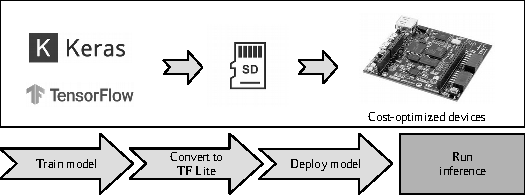
\includegraphics[width=0.5\textwidth]{../figures/workflow.pdf}
	\caption{The workflow of our approach on embedded FPGAs.}
	\label{fig:workflow}
\end{figure}

To operate the proposed system, the user trains a custom CNN model using TensorFlow or Keras, then this model is converted into a TensorFlow Lite, finally, the model is stored in a micro SD card memory and inserted in the system slot, see \Fig{fig:workflow}.

Our main contributions are as follows:
\begin{enumerate}
	\item We develop a hardware/software co-design framework targeting low-power, resource-limited embedded FPGAs for floating-point CNNs. This is a scalable and fully parameterized architecture integrated with TensorFlow Lite that allows hardware design exploration.
	\item We present a customizable tensor processor (TP) as a dedicated hardware accelerator. This design computes \emph{Conv2D} and \emph{DepthwiseConv2D} tensor operations employing a pipelined vector dot-product using hybrid custom floating-point and logarithmic approximation with parametrized on-chip memory utilization.
	\item We propose a quantize aware training method that maintains and increases inference accuracy with low-precision custom floating-point formats.
	\item We demonstrate the potential of the proposed architecture by addressing a design exploration with custom shallow CNN models using \emph{Conv2D} and \emph{DepthwiseConv2D} tensor operations. We evaluate compute performance and classification accuracy.
\end{enumerate}

The rest of the paper is organized as follows. Section~\ref{sec:related_work} covers the related work; Section~\ref{sec:background} introduces the background to \emph{Conv2D} and \emph{DepthwiseConv2D} tensor operations; Section~\ref{sec:system_design} describes the system design of the hardware/software architecture and the quantized aware training method; Section~\ref{sec:experimental_results} presents the experimental results thorough a design exploration flow; Section~\ref{sec:conclusions} concludes the paper.

This design exploration framework is available to the community as an open-source project at (\emph{hidden for double blinded review}).